\section{Recommendation systems}\label{sec:recommendation-systems}

In Denmark when using apps to guide your travels, you will have to choose between the different means of transport such
as: by car, train, bus, cycling or walking.
If you wanted to prioritize your climate footprint with these already existing apps you would have to research how much
a specific means of transportation pollutes.
Another situation is the economics of one's travel.
Instead of individuals having to calculate for themselves how much money they would spend on a specific travel type,
it could be done automatically.
To make it as easy as possible to make an informed decision for the users of our program, we want to automate many of
these calculations, such that the users can get an overview of their situation in a fast and easy way.

To accompany this, the authors will build a system that shows the routes that the user would want to travel by based on
their personal preferences.
This can also be called a recommendation system (RS).
RS is something we all use every day, when browsing a web shop, YouTube or other streaming services.
The goal of an RS is to sort through all available data and assume and present the most useful data to the user.
The close parallel there is between these RS and our problem solution gives rise to a segment explaining RS in more
detail.

A real world example of where this is used is in a movie recommender.
Movies are somewhat easy to classify, as one can look at the genres of different movies for example.
This type of RS works by filtering the movies through genres and is called ''content based filtering'' as seen in.

\begin{figure}
    \centering
    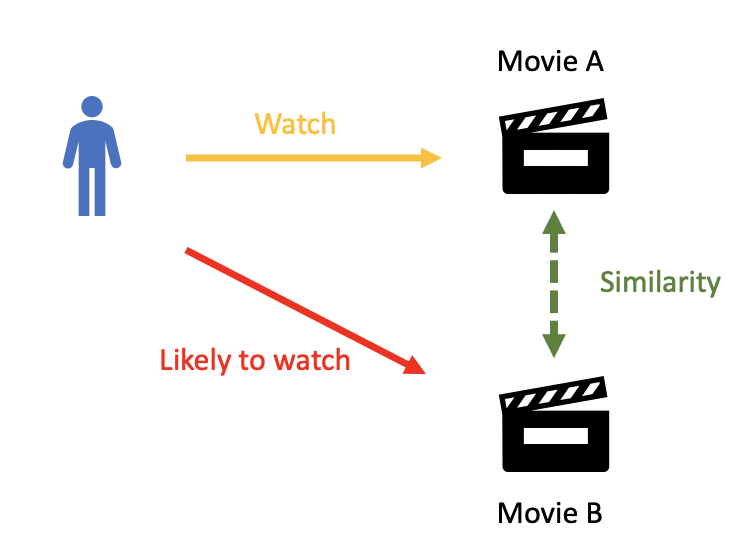
\includegraphics[width=\textwidth]{content-filtering}
    \caption{Content filtering. \cite{content_based_filtering}}
    \label{fig:figure3}
\end{figure}

An example would be user a watching an action movie, movie A, and the system would then remember user a's preferences
and recommend another action movie, movie B, to the user as seen in ~\ref{fig:figure3}.
This is a very simplified version of content filtering as they usually utilize multiple attributes from both the content
and the user.
In the context of a movie recommender this could be both the themes, the producer, the actors etc.
In content filtering, a user's history and interactions is used to create the profile for the RS to give suggestions.
Although content filtering is better than recommending random movies, it does not take human tendency to have changing
opinions and tastes into consideration.

Another type of filtering is Collaborative filtering (CF).
CF works by comparing users with each other.
This means that CF groups users by similarities in their watched movies, and then suggests movies from the users group,
as seen in~\ref{fig:figure4}.

\begin{figure}
    \centering
    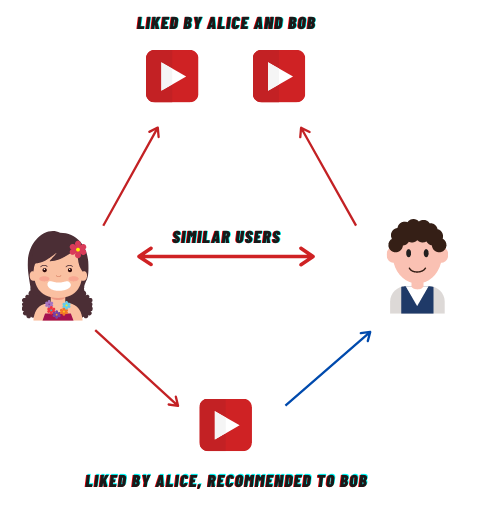
\includegraphics[width=\textwidth]{collaborative-filtering}
    \caption{Collaborative filtering. \cite{collaborative_filtering}}
    \label{fig:figure4}
\end{figure}

Using CF does not limit the recommendations to genres or other attributes that the program already know the user
watches.
It can also recommend things from other genres, which would not have been recommended by the content filter.
Generally for both these types of filters, they need a lot of information about both the user and the content.
This is however out of the scope of this project.
While content filters and collaborative filters are versatile in their use, the goal for this project is to use them to
recommend routes and make the user aware of both the monetary impact and the impact on our climate as well as
recommending the best routes.
In this context, it would be more logical and simpler to get the users preferences directly through what could be a
questionnaire, rather than relying on behavior analysis.
The attributes one could use for the filters are straight forward, as they could be climate impact, cost, time and
others.
This would however require some analysis to get more useful data out of the routes we generate.
Using a weighted system to measure the results of our program would allow us to choose a specified amount from the top,
and by doing this we will have chosen the most relevant for the users.
